\documentclass[12pt,a4paper]{report}
\usepackage[margin= 2.828cm]{geometry}
\usepackage[utf8]{inputenc}
\usepackage{amsfonts}
\usepackage{amsmath}
\usepackage{amssymb}
\usepackage{graphicx}
\usepackage{commath}
\usepackage{setspace}
\usepackage{mathtools,amsthm}
\usepackage{hyperref}
\usepackage{pgfplots}


\DeclareMathOperator{\deriv}{d}
\newcommand{\ihat}{\boldsymbol{\hat{\imath}}}
\newcommand{\jhat}{\boldsymbol{\hat{\jmath}}}
\newcommand{\khat}{\boldsymbol{\hat{\kmath}}}
\newcommand{\ehat}{\boldsymbol{\hat{e}}}
\newcommand{\dott}{\boldsymbol{\cdot}}

\newtheoremstyle{thms}% name
{}%         Space above, empty = `usual value'
{}%         Space below
{\itshape}% Body font
{}%         Indent amount (empty = no indent, \parindent = para indent)
{\bfseries}% Thm head font
{.}%        Punctuation after thm head
{\newline}% Space after thm head: \newline = linebreak
{}%         Thm head spec

\newtheoremstyle{defns}% name
{}
{}
{}
{}
{\bfseries}
{.}
{\newline}
{}

\theoremstyle{thms}
\newtheorem{theorem}{Theorem}[section]
\newtheorem{corollary}{Corollary}[theorem]
\newtheorem{lemma}[theorem]{Lemma}
\newtheorem{aside}{Aside}[section]

\theoremstyle{defns}
\newtheorem{definition}{Definition}[section]
\newtheorem{example}{Example}[section]

\title{An Introduction to Fourier Analysis}
\author{Michael Babb}
\date{}

\begin{document}
\maketitle

\begin{figure}
    \centering
    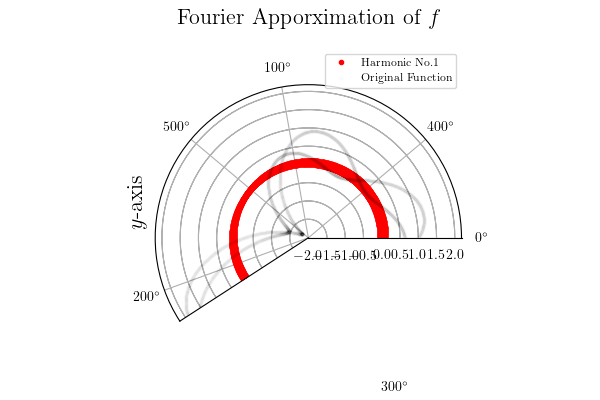
\includegraphics[width=0.5\textwidth]{assets/fourier.png}
\end{figure}


\newpage

\tableofcontents{}
\newpage

\section{Introduction}
The study of Fourier analysis has seen use in an wide array of topics such as spectrum/frequency analysis, ordinary/partial differential equation analysis, data compression, et infinitum. An assuredly incredibly useful field of study, as it allows one to potentially decompose an otherwise complex function, $f$, into a sum of simple sinusoids of varying period and amplitude. This analysis is then therein composed of two primary concepts: Fourier series and the Fourier transform. The former is the notion mentioned above: decomposing a function, $f$, into a sum of sinusoidal waves. Through this process of decomposition, one discovers the latter concept above, the Fourier transform: which, in turn, describes the amplitude and phase of each sinusoid that $f$ is therein composed.

The series of equations that from which these two concepts spawn can be seem rather daunting to the first time reader: infinite integrals and sums, complex exponentials; all of which being represented thereon the examination of the Fourier transform, and its complement and origin, Fourier series. However, when understood in all of its entirety, these two concepts become remarkably intuitive and understandable. One may gain this intuition rather quickly without the use of mathematical rigor, as the underlying notion of Fourier series and transform is rather straightforward:

\begin{description}
    \item[Fourier Series]
          One takes a given set of data, most often a function, and then represents that set of data using sinusoidal waves.

    \item[Fourier Transform]
          One takes a given set of data, and "plucks out" the sinusoidal waves that the preceding Fourier series was composed of.
\end{description}

Though the above are decidedly straightforward, and comparatively accurate representations of each mathematical concept, they both leave much to be desired. To attempt mathematical description of Fourier series and the Fourier transform then requires substantially more effort, insofar that the mathematics involved is fairly complex. Not complex in terms of topic, the mathematics involved is, in scope, comparatively understandable: rather, complex in terms of prerequisite knowledge required. This higher barrier of entry admits a higher reward, however: for if one understands each component of Fourier series and transform, one implicitly then has command over a wide array of elementary mathematics.

The concepts mentioned heretofore may thus be accurately described from many mathematical perspectives: it is then the aim of this paper to focalize on two of the aforementioned perspectives: from both the lens of linear algebra, and then complex analysis.

To do so, we'll first motivate Fourier analysis with a concrete example: this is achieved by looking back directly to its inception: using a published work by Fourier himself, we will derive Fourier series using Fourier's "Théorie analytique de la chaleur". The outline of the proceeding paper will be thusly described as: Chapter 1 will contain this derivation; chapter 2 will then expand on this derivation, and reveal its connection to both linear algebra and complex analysis. Finally, chapters 3 and 4 will be dedicated to corporeal applications of Fourier analysis: this will be achieved through demonstration of image convolution, tidal frequency analysis. These programmatic examples will be implemented in both Python and C++ and utilize algorithms developed by the author.

It is a frustration of the author that, whereupon reading mathematical texts and one comes across some arbitrarily complex theorem, it is often the case that the proof of said theorem is then "left as an exercise to the reader". To counter this minor annoyance, it will then be the effort of the author to, whenever a theorem is offered, either provide a proof directly, or direct the reader to a proof of said theorem in another text. This will be done in an attempt to make the paper as inclusive as possible, with all the necessary knowledge of each concept built upon the former.

However, one must have a set of basal mathematical knowledge before reading the proceeding paper to fully grasp each concept mentioned and used within. The following concepts are then listed as prerequisites for full understanding:

\begin{enumerate}
    \item Basic knowledge of linear algebra. Particularly surrounding the notions of vector spaces and linear transformations.
    \item A firm understanding of ordinary differential equations, and a basic knowledge of partial differential equations.
    \item Basic knowledge of complex analysis.
    \item A firm command of elementary calculus.
\end{enumerate}

Additionally, knowledge of real analysis and basic set theory will surely prove helpful throughout the text, though they are not prerequisite in any way.

For theorems involving said prerequisite material, they will be labeled then as "definitions", rather than "theorems", as they are most likely known already to the reader.



\chapter{Origin and Derivation}

Jean-Baptiste Joseph Fourier (21 March 1768 – 16 May 1830), was a pioneer in the fields of harmonic analysis and heat propagation, and creator of the field which bears his name: Fourier analysis. Throughout his colorful career as mathematician and Prefect, Fourier published many revolutionary mathematical treatises; but it is however his 1822 publication, "Théorie analytique de la chaleur", or "The Analytic Theory of Heat", that is indubitably one his most important: for it is in this publication that Fourier introduces the notion that \textit{any} well-behaved function can be thereby expanded into a series of sinusoidal waves. Though this has proven to not be a general truth; notwithstanding, many functions, provided certain conditions are met, can be expanded into an infinite sum of sinusoids.

Utilizing excerpts from Fourier's, "Théorie analytique de la chaleur", we shall derive Fourier series in a manner quite similar to Fourier himself. Before this, however, let's take a peek at the end result we so desire:

Given a well behaved function, $f(x)$, $f$, can thereby be expanded into the following infinite series:
\begin{theorem}[Fourier Series of a well-behaved $f$]
    \begin{equation}
        f(x) = \sum_{n=-\infty}^{\infty} c_ne^{inx}
    \end{equation}
\end{theorem}

This will be proved in chapter II.

\section{Fourier's Problem}
All of the content introduced in Fourier's "Théorie analytique de la chaleur" is fascinating, however it is Chapter III, "Propagation of Heat in an infinite rectangular solid", that is of most relevance to us; the first section, Fourier states the problem at hand:

\begin{quote}"Suppose a rectangular plate $BAC$, of infinite length, to be heated at its base $A$, and to preserve at all points of the base a constant temperature 1, whilst each of the two infinite sides $B$ and $C$, perpendicular to $A$, is submitted also at every point to a constant temperature 0; it is then required to determine what must be the stationary temperature at any point of the plate." \cite{heat_fourier}
\end{quote}

Hereof is a description of a partial differential equation describing the heat flow over a three dimensional lamina of infinite length. Fourier imposes Dirichlet boundary conditions thereon:

\begin{quote}
    "...The solid $BAC$ must 1st, satisfy the equation (a); 2nd, become nothing when we substitute $\pm\dfrac{\pi}{2}$ for $y$, whatever the value of $x$ may be; 3rd, must be equal to unity when we suppose $x=0$
    and $y$ to have any value between $[-\dfrac{\pi}{2}, \dfrac{\pi}{2}]$." \cite{heat_fourier}
\end{quote}

Translated symbolically, both the boundary conditions and partial differential equation have the form:

\begin{align}
     & u(x, \pm\dfrac{\pi}{2}) = 0                          \\
     & u(0, y) = 1, y \in [-\dfrac{\pi}{2}, \dfrac{\pi}{2}] \\
     & u(x, y), x\to\infty, y\to\infty = 0
\end{align}

Starting from the general heat equation $u_t = \Delta u$ where $u = u(x, y, t)$, the steady-state condition $u_t = 0$ yields:
\begin{equation}
    \dfrac{\partial^2 u(x, y)}{\partial x^2} + \dfrac{\partial^2 u(x, y)}{\partial y^2} = 0
    \label{eq:f1}
\end{equation}

That is, $u$ is not a function of time; it is unchanging in this dimension. Equation \eqref{eq:f1} can be written succinctly as:
\begin{equation}
    \Delta u(x, y) = 0
    \label{eq:f2}
\end{equation}

\begin{aside}
    Where $\Delta u$ represents the Laplacian of $u$. Recall the laplacian in merely the divergence of the gradient of a given function. Thus, all of the following forms are equivalent:
    \begin{align}
        \dfrac{\partial^2 u(x, y)}{\partial x^2} + \dfrac{\partial^2 u(x, y)}{\partial y^2} & = 0 \\
        u_{xx} + u_{yy}                                                                       & = 0 \\
        \Delta u(x, y)                                                                      & = 0 \\
        \nabla \dott \nabla u(x, y)                                                         & = 0 \\
        \nabla^2u(x, y)                                                                     & = 0
    \end{align}
\end{aside}

\section{A Solution}
To solve \eqref{eq:f2}, we'll as proceed Fourier did, utilizing separation of variables. To do as such, we will make the assumption that $u(x, y)$ may be represented by the product of two potential functions as follows:
\begin{align}
    u      & = X(x)Y(y)\label{eq:assum1} \\
    u_{xx} & = X''(x)Y(y)\label{eq:xx}   \\
    u_{yy} & = X(x)Y''(y)\label{eq:yy}
\end{align}

Substituting \eqref{eq:xx} and \eqref{eq:yy} into \eqref{eq:f2}:
\begin{equation}
    \dfrac{X''(x)}{X(x)} = -\dfrac{Y''(y)}{Y(y)}
    \label{eq:f3}
\end{equation}

Notice the following: as X(x) changes, Y(y) does as well, but only in accordance to x; the inverse holds as well. If our assumption of \eqref{eq:assum1} is valid, then we must thereby conclude that both the left and right sides of \eqref{eq:f3} equal a constant. We'll call this constant $\lambda$, and implement in the following manner, yielding two separate equations:

\begin{align}
    \dfrac{X''(x)}{X(x)} & = \lambda  \\
    \dfrac{Y''(y)}{Y(y)} & = -\lambda
\end{align}

Which is represented by the following two ordinary differential equations:
\begin{align}
    X'' - \lambda X & = 0 \label{eq:sturm1} \\
    Y'' + \lambda Y & = 0 \label{eq:sturm2}
\end{align}

Moreover, both of the above are Sturm-Liouville problems. Let us take a brief detour from Fourier's path, and analyze the above equations through the lens of Sturm-Liouville theory.

\subsection{Sturm-Liouville Theory}
Recall the standard form of the classical Sturm-Liouville differential equation:
\begin{equation}
    \dfrac{\deriv}{\deriv{x}}[p(x) \dfrac{\deriv{y}}{\deriv{x}}] + y(q(x) + \lambda w(x)) = 0
\end{equation}

Transforming \eqref{eq:sturm1} and \eqref{eq:sturm2} into the canonical Sturm-Liouville form:
\begin{align}
    \dfrac{\deriv}{\deriv{x}}[p(x) X'] + X(q(x) + \lambda w(x)) & = 0 \\
    \dfrac{\deriv}{\deriv{y}}[p(y) Y'] + Y(q(y) + \lambda w(y)) & = 0
\end{align}

Where:

\begin{align}
    p(x) & = p(y) = 1 \\
    q(x) & = q(y) = 0 \\
    w(x) & = -1       \\
    w(y) & = 1
\end{align}

From Sturm-Liouville theory, we have the following theorem:

\begin{theorem}[Eigen-function Orthogonality]
    If one has the following Sturm-Liouville differential equation, with predefined Dirichlet boundary conditions:
    \begin{align}
         & \dfrac{\deriv}{\deriv{x}}[p(x) \dfrac{\deriv{y}}{\deriv{x}}] + y(q(x) + \lambda w(x)) = 0 \\
         & y(a) = y(b) = 0
    \end{align}

    And if the above produces at least two distinct eigen-function-value pairs:
    \begin{align}
        y_n, \lambda_n \\
        y_m, \lambda_m
    \end{align}

    Then $y_n$ and $y_m$ are said to be orthogonal on the interval $[a, b]$:

    \begin{equation}
        \int_{a}^{b} y_ny_mw(x) \deriv{x} = 0
        \label{eq:ortho-strum}
    \end{equation}
    \label{thm:sturm_proof}
\end{theorem}

Let's prove it:

\begin{proof}[Proof of Eigen-function Orthogonality]
    Assume that the solution to:
    \begin{align}
         & \dfrac{\deriv}{\deriv{x}}[p(x) y_n'] + y(q(x) + \lambda w(x)) = 0 \\
         & y(a) = y(b) = 0
    \end{align}

    yields distinct eigen-function-value pairs of:

    \begin{align}
        y_n, \lambda_n \\
        y_m, \lambda_m
    \end{align}

    Plugging these then into the above yields:
    \begin{align}
         & \dfrac{\deriv}{\deriv{x}}[p(x)y_n'] + y_n(q(x) + \lambda_n w(x)) = 0 \label{eq:sturm_proof1} \\
         & \dfrac{\deriv}{\deriv{x}}[p(x)y_m'] + y_m(q(x) + \lambda_m w(x)) = 0 \label{eq:sturm_proof2}
    \end{align}

    Multiplying \eqref{eq:sturm_proof1} by $y_m$, \eqref{eq:sturm_proof2} by $-y_n$, and then adding the respective equations together yields:
    \begin{align}
         & \dfrac{\deriv}{\deriv{x}}[p(x)y_n']y_m - 	\dfrac{\deriv}{\deriv{x}}[p(x)y_m']y_n + y_ny_m(q(x) + \lambda_n w(x)) - y_ny_m(q(x) + \lambda_m w(x)) = 0 \\
         & \dfrac{\deriv}{\deriv{x}}[p(x)y_n']y_m - 	\dfrac{\deriv}{\deriv{x}}[p(x)y_m']y_n + (\lambda_n - \lambda_m)(y_ny_mw(x)) = 0                           \\
         & (\lambda_n - \lambda_m)(y_ny_mw(x)) = 	\dfrac{\deriv}{\deriv{x}}[p(x)y_m']y_n - \dfrac{\deriv}{\deriv{x}}[p(x)y_n']y_m \label{eq:strum_proof3}
    \end{align}

    We wish to prove the orthogonality of $y_n$ and $y_m$, which implies that the left hand of \eqref{eq:strum_proof3} must be integrated from $a$ to $b$. Therefore, we will integrate both sides of the above to form:
    \begin{align}
        (\lambda_n - \lambda_m)\int_{a}^{b}y_ny_mw(x) \deriv{x} = \int_{a}^{b}\dfrac{\deriv}{\deriv{x}}[p(x)y_m']y_n - \dfrac{\deriv}{\deriv{x}}[p(x)y_n']y_m \deriv{x}
    \end{align}

    Integrating the right hand side of the above by parts yields:
    \begin{align}
        (\lambda_n - \lambda_m)\int_{a}^{b}y_ny_mw(x) \deriv{x} & = p(x)y_ny'_m \Big|_a^b - p(x)y_my_n' \Big|_a^b - \int_{a}^{b}p(x)y_n'y_m' \deriv{x} + \int_{a}^{b}p(x)y_n'y_m' \deriv{x} \\
        (\lambda_n - \lambda_m)\int_{a}^{b}y_ny_mw(x) \deriv{x} & = p(x)y_ny'_m \Big|_a^b - p(x)y_my_n' \Big|_a^b
    \end{align}

    Since the boundary condition of $y(a) = y(b) = 0$ was given, the left hand side vanishes. This then gives the following:
    \begin{equation}
        (\lambda_n - \lambda_m)\int_{a}^{b}y_ny_mw(x) \deriv{x} = 0
    \end{equation}

    The only solution wherein this equality holds is if the integral equals to zero. This stems from our condition that $\lambda_n$ and $\lambda_m$ were distinct eigen values; thus, $\lambda_n \neq \lambda_m$

    Finally, we arrive at our ending statement:
    \begin{equation}
        \int_{a}^{b}y_ny_mw(x) \deriv{x} = 0
    \end{equation}
\end{proof}

A natural question arises: do the eigenfunctions of a Sturm-Liouville problem form a \textit{complete} set? That is, can any sufficiently well-behaved function be represented as a series of these eigenfunctions? The answer is affirmative:

\begin{theorem}[Completeness of Sturm-Liouville Eigenfunctions]
    Let $\{y_n\}_{n=1}^{\infty}$ be the eigenfunctions of a regular Sturm-Liouville problem on $[a, b]$ with weight function $w(x) > 0$. Then the set $\{y_n\}$ is complete in $\mathbf{L}^2_w[a, b]$: for any square-integrable function $f$ on $[a, b]$,
    \begin{equation}
        f(x) = \sum_{n=1}^{\infty} c_n y_n(x), \quad c_n = \dfrac{\int_a^b f(x)y_n(x)w(x)\deriv{x}}{\int_a^b y_n^2(x)w(x)\deriv{x}}
    \end{equation}
    where the convergence is in the $\mathbf{L}^2_w$ sense.
    \label{thm:sturm_completeness}
\end{theorem}

The proof of this theorem is beyond the scope of this paper; the interested reader is directed to \cite{courant_hilbert} for a thorough treatment. This completeness result is precisely what justifies the Fourier series representation: the trigonometric functions that emerge from our particular Sturm-Liouville problem form a complete orthogonal system.

Indeed, equation \eqref{eq:sturm1} does not satisfy this form, as the original boundary conditions given by Fourier were specified an interval only for $y$. However, equation \eqref{eq:sturm2} \textit{does}: thus, the solution of \eqref{eq:sturm2} must produce a linearly independent set of orthogonal eigen basis functions. This will be key insight into our solution to the original PDE given by Fourier. Let us return now to Fourier's original path.

\subsection{Continuing On Fourier's Path}
Notice the constant $\lambda$ has three possible states: positive, negative and zero.

Let's look at each case for both equation listed above:

\begin{align}
    X(x) & = \begin{cases}
        Ax + B                                         & \lambda = 0 \\
        Ae^{i\sqrt{\lambda}x} + Be^{-i\sqrt{\lambda}x} & \lambda < 0 \\
        Ae^{\sqrt{\lambda}x} + Be^{-\sqrt{\lambda}x}   & \lambda > 0
    \end{cases} \\
    Y(y) & = \begin{cases}
        Cy + D                                         & \lambda = 0 \\
        Ce^{\sqrt{\lambda}y} + De^{-\sqrt{\lambda}y}   & \lambda < 0 \\
        Ce^{i\sqrt{\lambda}y} + De^{-i\sqrt{\lambda}y} & \lambda > 0
    \end{cases}
\end{align}

Notice the above complex solutions can be simplified into the following respective forms:
\begin{enumerate}
    \item $A\cos(\sqrt{\lambda}x) + B\sin(\sqrt{\lambda}x)$
    \item $C\cos(\sqrt{\lambda}y) + D\sin(\sqrt{\lambda}y)$
\end{enumerate}

For this particular problem, $\lambda$ must be positively valued. To see why, and to determine its precise form, we apply the boundary conditions. Consider $Y(y) = C\cos(\sqrt{\lambda}y) + D\sin(\sqrt{\lambda}y)$ with $Y(\pm\pi/2) = 0$. From $Y(\pi/2) = 0$ and $Y(-\pi/2) = 0$, adding and subtracting these conditions yields:
\begin{align}
    2C\cos(\sqrt{\lambda}\pi/2) & = 0 \\
    2D\sin(\sqrt{\lambda}\pi/2) & = 0
\end{align}

For a non-trivial solution, at least one of $C$ or $D$ must be nonzero. As we seek even solutions (consistent with $u(0, y) = 1$ being even), we take $D = 0$ and require $\cos(\sqrt{\lambda}\pi/2) = 0$, which gives $\sqrt{\lambda}\pi/2 = (2n+1)\pi/2$, hence:
\begin{equation}
    \lambda = (2n + 1)^2, \quad n \in \mathbb{N}
\end{equation}

Using again the boundary conditions, it follows then that $X(x)$ and $Y(y)$ are equal to the following:
\begin{align}
    X(x) & = B_ne^{-(2n+1)x}                 \\
    Y(y) & = C_n\cos{(2n+1)y}\label{eq:yofy}
\end{align}

As $\lambda$ can take on any integer value greater than one, a general solution must be an infinite sum representing $X(x)Y(y)$. The solution is thus:
\begin{align}
    u(x, y) & = X(x)Y(y)                                         \\
    u(x, y) & = \sum_{n=0}^{\infty} c_ne^{-(2n+1)x}\cos((2n+1)y)
\end{align}

Notice the values of $B_n$ and $C_n$ were combined into one ultimate constant, $c_n$.\\

Wonderful, a general solution! But what of the constants $c_n$? Fourier uses a series (no pun intended) of ingenious and rather complicated steps to calculate a closed form expression for them. Notwithstanding the above, we can bypass much of the tedious calculation by using the results of our detour into Sturm-Liouville theory. Recall that the solution to equation \eqref{eq:sturm2} was guaranteed to be orthogonal on the interval from $[-\dfrac{\pi}{2}, \dfrac{\pi}{2}]$. We'll exploit this orthogonality using the following technique, which was subsequently used later by Fourier himself; "Fourier's trick", see chapter III, section IV of "Théorie analytique de la chaleur". First, we will impose the boundary condition of $u(0, y) = 1, y \in [-\dfrac{\pi}{2}, \dfrac{\pi}{2}]$:

\begin{equation}
    1 = \sum_{n=0}^{\infty} c_n\cos((2n+1)y)
    \label{eq:f4}
\end{equation}

\begin{figure}[h]
    \centering
    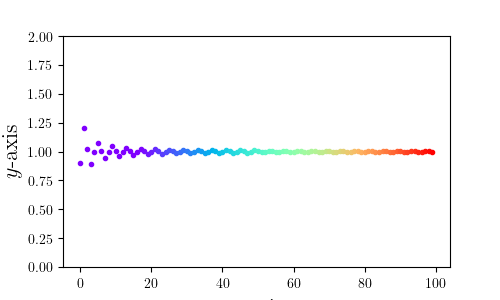
\includegraphics[width=0.8\textwidth]{assets/partial_sums_of_1.png}
    \caption{The partial sums of the above equation converging to 1}
\end{figure}

If we multiply both sides of \eqref{eq:f4} by $\cos((2m+1)y)$, and then integrate over our original boundary interval, we achieve the following:
\begin{equation}
    \int_{-\dfrac{\pi}{2}}^{\dfrac{\pi}{2}} \cos((2m+1)y)\deriv{y} = \int_{-\dfrac{\pi}{2}}^{\dfrac{\pi}{2}} \left[\sum_{n=0}^{\infty} c_n\cos((2n+1)y)\right]\cos((2m+1)y)\deriv{y}
    \label{eq:dotted1}
\end{equation}

Since our assumption is that the sum on the right is convergent, we may switch the summation and integrals signs (thanks, Fubini!), yielding:
\begin{equation}
    \int_{-\dfrac{\pi}{2}}^{\dfrac{\pi}{2}} \cos((2m+1)y)dy = \sum_{n=0}^{\infty}c_n\int_{-\dfrac{\pi}{2}}^{\dfrac{\pi}{2}}\cos((2m+1)y)\cos((2n+1)y)dy
\end{equation}

If the $m \neq n$, the integral on the right vanishes, which is exactly what was foretold by our results from Sturm-Liouville theory. However if $m = n$, the integral $\neq 0$. Thus, the sum on the right vanishes down to $m$. We'll now evaluate both integrals, and solve for $c_n$:
\begin{align}
    \dfrac{2(-1)^m}{2m+1} & = c_m \dfrac{\pi}{2} \\
    c_m                   & = \dfrac{4(-1)^m}{(2m + 1)\pi}
\end{align}

Which is simply fantastic: we've found a closed form expression for all values of $c$. Notice that the same result was achieved by Fourier on page 144 in "Théorie analytique de la chaleur", but took Fourier nearly six pages of complicated arithmetic to prove. What a time save!

Putting this together, we now have the following Fourier cosine series representation for the constant 1:
\begin{equation}
    1 = \sum_{n=0}^{\infty} \dfrac{4(-1)^n}{2\pi n + \pi}\cos((2n+1)y), y \in [-\dfrac{\pi}{2}, \dfrac{\pi}{2}]
    \label{eq:seriesfor1}
\end{equation}

And a definition, which may be extrapolated from the original problem byway of boundary change:

\begin{definition}[Fourier Cosine Series]
    \begin{align}
         & f(y) = \sum_{n=0}^{\infty} c_n\cos(ny)  \\
         & y \in [-\dfrac{\pi}{2}, \dfrac{\pi}{2}]
        \label{eq:fourier_cosine_series}
    \end{align}
\end{definition}

An amazing result from this is the Leibniz formula for $\pi$ when y = 0:

\begin{equation}
    \dfrac{\pi}{4} = \sum_{n=0}^{\infty} \dfrac{(-1)^n}{2n+1}
\end{equation}

Finally, our solution for $u(x, y)$, satisfying all of the boundary conditions is the following:

\begin{equation}
    u(x, y) = \sum_{n=0}^{\infty} \dfrac{4(-1)^n}{2\pi n + \pi}e^{-(2n + 1)x}\cos((2n+1)y)
\end{equation}

\section{Potentially Generalizing The Result}

Fourier continues onward and generalizes the results of Chapter III, section IV of, "Théorie analytique de la chaleur", but his methodology is exceedingly arithmetically complex and rather terse. We shall then again for the final time diverge from Fourier's path, and rather view the notion of Fourier Analysis from two separate viewpoints: linear algebra and complex analysis.\\

Upon cursory examination of the above material, one may notice straight away similarities with several topics from each respective discipline:

In equation \eqref{eq:fourier_cosine_series}, $f(y)$ is being expressed as a linear combination of cosine terms, multiplied by various constants, $c_n$. This looks shockingly similar to both then power series, and vector expression via an orthogonal basis. Not so surprising, however, because the above concepts and equation\eqref{eq:fourier_cosine_series} are one in the same. Indeed, another similarity can also be surmised through our Sturm-Liouville adventure, whereon the concept of orthogonality is expressed explicitly: as one may guess, this was equivalent to the inner product operation that one sees in linear algebra.

The above two assertions will be explained formally in the proceeding chapters. First, through linear algebra, then through complex analysis (Laurent series!). Onward to the next chapter!



\chapter{Lens I: Linear Algebra}
\begin{figure}[h]
    \centering
    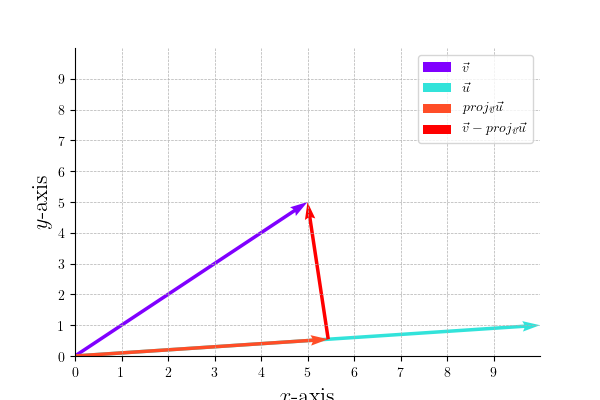
\includegraphics[width=0.6\textwidth]{assets/projection.png}
    \caption{Vector Projection of vectors $\vec{u}$ and $\vec{v}$. Recall that vector or subspace projection can be viewed as a way to discern "how much" of one vector is represented in another.}
    \label{fig:proj}
\end{figure}



\section{An Appeal to Intuition}
Recall, that a vector, $\vec{u}$, of dimension N, located within the span of some arbitrary orthonormal basis, $B^T$, may be thereupon written as a linear combination of basis vectors therein $B^T$ as such:
\begin{equation}
    \vec{u} = \sum_{n=0}^{N} c_n\ehat_n
\end{equation}


Where the coefficients $c_n$ may be found by:
\begin{align}
    \langle \vec{u}, \ehat_n \rangle   & = \sum_{n=0}^{N} c_n\langle \vec{u}, \ehat_n \rangle \\
    \langle \vec{u}, \ehat_n \rangle   & = c_n                                                \\
    \mathnormal{proj}_{\ehat_n}\vec{u} & = c_n
\end{align}
This projection operation is taking the original vector, $\vec{u}$, and \textit{transforming} its original basis to the newly defined basis, $B^T$.\\


Recall then the euclidean inner product for two arbitrary vectors of dimension $N$, $\vec{u}$ and $\vec{v}$:

\begin{definition}[Euclidean Inner Product]
    \begin{equation}
        \langle \vec{u}, \vec{v} \rangle = \sum_{n=0}^{N} \vec{u}_n\vec{v}_n
    \end{equation}
\end{definition}

Notice the vector space that one is operating in is $\mathbb{R}^N$. The above logic applies to vectors of dimension $N$, but what if one wished to apply the same logic to continuous functions? How does this translate? As a first attempt, one may think of a continuous function as a vector of infinite dimension. Let's see a discrete time example of this:

\begin{example}
    Take a function, $f(x)$, which is valid on the interval $[-1, 1]$. $f$ is essentially being sampled continuously, infinitely many times, from the line $[-1, 1]$ in  $\mathbb{R}$.

    Let us now descritize this example, and instead sample $f$ in increments of $0.5$. We would then be sampling $f$ at: $(-1, -0.5, 0, 0.5, 1)$. If we took the responses of $f$ at the given interval steps above, we could then store said responses in a vector, $\vec{f}$:

    \begin{equation}
        \vec{f} =
        \begin{bmatrix}
            f(-1)   \\
            f(-0.5) \\
            f(0)    \\
            f(0.5)  \\
            f(1)
        \end{bmatrix}
    \end{equation}

    If we instead sample $f$ in increments of $\dfrac{1}{N}$, where $N\to\infty$, we can see:

    \begin{equation}
        \vec{f} =
        \begin{bmatrix}
            f(-1)                \\
            f(-1 + \dfrac{1}{N}) \\
            \vdots               \\
            f(1)
        \end{bmatrix}
    \end{equation}

    Which, in the limit, is exactly equal to $f(x)$ at any point in the domain of $[-1, 1]$. And notice, this choice of domain was entirely arbitrary. Instead, we could sample $f$ across the entirety of $\mathbb{R}$, and then have a valid $\vec{f}$ vector for any $x$ in $[-\infty, \infty]$.
\end{example}


\begin{figure}
    \centering
    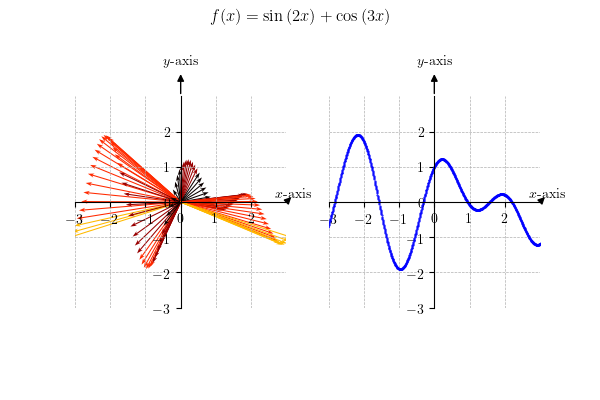
\includegraphics[width=0.6\textwidth]{assets/f_as_vec.png}
    \caption{Vector representation of a given $f$. The intensity of the vector is proportional to the value of $f$ at that point.}
\end{figure}

Before we can extend the concept of vectors to continuous functions (vectors of then infinite dimension), we'll need a few definitions to build up to the final result: $\mathbf{L}^2$ Hilbert space. To do so, we will move downwards in abstraction using the following hierarchy:\\

Metric spaces $\rightarrow$ Normed vector spaces $\rightarrow$ Banach spaces $\rightarrow$ Inner product spaces $\rightarrow$ Hilbert space\\

A Banach space is a complete normed vector space: one in which every Cauchy sequence converges. A Hilbert space additionally requires an inner product that induces the norm. This distinction is important: $\mathbf{L}^p$ for $p \neq 2$ is Banach but not Hilbert.

\begin{aside}
    It is assumed that the reader is aware of the definition of an inner product space, thereby the definition is implicit therein.
\end{aside}

The above abstractions are very broad topics, of which are not suitable for proper analysis in one given paper, nor are they our focus here: we merely require small bits of information from each. As such, we will not provide much detail regarding said concepts: just enough so that the reader may have a general understanding of the requisite material required for Hilbert space.

\section{Metric Spaces}
A metric space is a set, $\mathbf{M}$, that has a notion of distance between any two two-tuples of points therein $\mathbf{M}$. This distance can be defined by a distance function, or $\mathit{metric}$, $d$.

\begin{definition}[Metric Space]
    Define $(\mathbf{M}, d)$, where  $\mathbf{M}$ is a set, and $d$ is a $\mathit{metric}$ on $\mathbf{M}$. $d$ is then:  $\mathbf{M} \times \mathbf{M} \rightarrow \mathbb{R}$, such that $\forall x, y, z \in \mathbf{M}:$

    \begin{enumerate}
        \item $d(x, y) \geq 0$
        \item $d(x, y) = 0 \iff x = y$
        \item $d(x, y) = d(y, x)$
        \item $d(x, y) \leq d(x, z) + d(z, y)$
    \end{enumerate}
\end{definition}

Let's look a two examples of metrics commonly used:

\begin{definition}[The Euclidean, or $\ell^n$, Metric]
    Define $d$: $\mathbb{R}^n \times \mathbb{R}^n \rightarrow \mathbb{R}$ by:

    \begin{equation}
        d(x, y) = \sqrt{\sum_{k=0}^{N} (x_k - y_k)^2}
    \end{equation}

    Where:
    \begin{align}
        x & = (x_0, x_1 \dots x_N) \\
        y & = (y_0, y_1 \dots y_N)
    \end{align}


\end{definition}

Notice when $n = 1$, $d(x, y)$ reduces to the absolute difference between two points, $x, y$.

Different metrics may thereby be used on the same set. Take the $\ell^1$ metric on $\mathbb{R}^2$:


\begin{definition}[The $\ell^1$, Metric on $\mathbb{R}^2$]
    Define $d$: $\mathbb{R}^2 \times \mathbb{R}^2 \rightarrow \mathbb{R}$ by:

    \begin{equation}
        d(x, y) = |x_0 - y_0| + |x_1 - y_1|
    \end{equation}

    Where:
    \begin{align}
        x & = (x_0, x_1) \\
        y & = (y_0, y_1)
    \end{align}
\end{definition}

To further our descent into normed vector, spaces, we will use a special case of a metric space: the Cauchy metric space.

First, recall the definition of a Cauchy sequence in the context of metric spaces:

\begin{definition}[Cauchy Sequence]
    For a given metric space, $\mathbf{M}$, defined with a metric, $d$, a sequence:
    \begin{equation}
        x_0, x_1 \dots x_n
    \end{equation}
    is said to be Cauchy if for every $\epsilon > 0$ there exists $N \in \mathbb{Z}^+$ such that for all $m, n > N$, $d(x_m, x_n) < \epsilon$
\end{definition}

Concretely, a sequence is said to be Cauchy if the distance between two two-tuples of points within a metric space, $\mathbf{M}$, gets smaller and smaller, such that there possibly exists some limit, $L$, that the sequence converges to. This leads us into the definition of a Cauchy, or complete, metric space:

\begin{definition}[Cauchy Metric Space (Complete Metric Space)]
    A given metric space, $\mathbf{M}$, defined with a metric, $d$, is said to be Cauchy if:

    \begin{enumerate}
        \item Every sequence within $\mathbf{M}$ is convergent to a limit.
        \item Each respective limit lies within $\mathbf{M}$.
    \end{enumerate}
\end{definition}

For further reading regarding metric spaces, and subsequent proof of the above definitions, see \cite{kaplansky_basic}.\\

Generally, operations on metric spaces are restricted only to modifications of the metric: no other algebraic manipulations are permitted. To algebraically operate a space with a given metric, we will turn our attention now to normed vector spaces.

\section{Normed Vector Spaces}

Using the above notion of a metric, or distance within a metric space, we will be able to define a normed vector space. Note that the metric on a vector space is typically derived from its respective norm.

\begin{definition}[Normed vector spaces]
    Define $(\mathbf{X}, ||\cdot||)$, where $\mathbf{X}$ is a vector space and $||\cdot||$ is a norm defined on $\mathbf{X}$. $||\cdot||$  is then:  $\mathbf{X} \rightarrow \mathbb{R}$ such that $\forall x, y \in  \mathbf{X}$:
    \begin{enumerate}
        \item $||x|| \geq 0$
        \item $||x|| = 0 \iff x = 0$
        \item $||cx|| = |c|\cdot||x||$
        \item $||x + y|| \leq ||x|| + ||y||$; Triangle Inequality.
    \end{enumerate}
\end{definition}



\begin{theorem}[Cauchy-Schwarz Inequality]
    If $\mathbf{X}$ is an inner product space with associated norm, $||\cdot||$, then $\forall x, y \in  \mathbf{X}$:

    \begin{equation}
        \langle x, y \rangle \leq ||x|\cdot|||y||
    \end{equation}
\end{theorem}

\begin{proof}
    Let $x$ and $y$ be arbitrary vectors located within an inner product space $\mathbf{X}$, that is defined with an associated norm of $||\cdot||$, where $\mathbf{X}$ is a field over either all of $\mathbb{R}$ or $\mathbb{C}$.

    Notice that if either $x$ or $y$ equals zero, the equality holds. Thus, we will ignore the case where either $x = 0$ or $y = 0$.

    Define a new vector, $z$ that is orthogonal to $y$. This is done by applying the Gram-Schmidt process:
    \begin{align}
        z & = x  - \dfrac{\langle x, y \rangle}{\langle y, y \rangle}y \\
        x & = z + \dfrac{\langle x, y \rangle}{\langle y, y \rangle}y
    \end{align}

    We then apply the Pythagorean theorem to yield:
    \begin{align}
        ||x||^2 & = ||z||^2 + \left|\dfrac{\langle x, y \rangle}{\langle y, y \rangle}\right|^2||y||^2 \\
                & = ||z||^2 + \dfrac{|\langle x, y \rangle|^2}{||y||^2}
    \end{align}

    Since $||z||^2 \geq 0$:

    \begin{align}
        \dfrac{|\langle x, y \rangle|^2}{||y||^2} \leq ||x||^2
    \end{align}

    The above then implies:

    \begin{align}
         & |\langle x, y \rangle|^2 \leq ||x||^2\cdot||y||^2 \\
         & |\langle x, y \rangle| \leq ||x||\cdot||y||
    \end{align}
\end{proof}

A proof of the Triangle Inequality may be easily derived using then the Cauchy-Schwarz Inequality. For further reading regarding the above topics, see \cite{holland_schwarz}\\

The above axioms make a great deal of sense when viewed through the lens of a metric. If a norm, $||x||$ is defined as a metric, $d(x, y)$ then certainly this distance is only 0 when d is zero. For an intuitive reasoning for the Triangle inequality:

Let $||x||$ be the distance from point A to B, and let $||y||$ be the distance from A to C. Certainly, the path from A to B to C is always longer than the direct path from A to C.\\

From the definition of a normed vector space, we arrive at the following (rather trivial) fact: a normed vector space is a prerequisite of an inner product space.

Collating all of the preceding information into one respective concept, we may now finally define Hilbert space.

\section{Hilbert Space}
We now have all of the tools required to properly define a Hilbert space! Without further ado:

\begin{definition}[Hilbert Space]
    Hilbert space, $\mathbf{H}$, is a real or complex inner product space that is additionally a Cauchy metric space w.r.t the distance function, $d$ defined by said inner product. The inner product is then defined as $\langle f, g \rangle$, with a norm defined as:
    \begin{equation}
        ||f|| = {\langle f, f \rangle}^{1/2}
    \end{equation}
\end{definition}

One can see now why the preceding sections were needed! All of the nice features of each component required to construct a Hilbert space is therein inherited by said space, which is great!\\

One may look at the definition and wonder what differentiates a Hilbert space from a standard real or complex inner product space. The key differentiating factor is thus: a Hilbert space is a Cauchy metric space, whilst an inner product space may be not. This is crucial, because this qualifier is the key to then extending the notion of finite dimensional vectors to ones of infinite dimension. Why? Let's look at an example:

Take a real inner product space, $\mathbf{X}$, defined with an inner product of:
\begin{equation}
    \langle f(x), g(x) \rangle = \int_{-\infty}^{\infty}f(x)g(x) \deriv{x}
\end{equation}

and defined with a norm (and subsequent metric) of:
\begin{equation}
    ||f(x)|| = 	\sqrt{\langle f(x), f(x) \rangle}
\end{equation}

Notice this metric lies within a $\ell^2$ metric space.\\

If $\mathbf{X}$ was a standard inner product space, there would be no guarantee that the above norm or inner product would converge. However, if $\mathbf{X}$ were a Hilbert space, then by definition, the above \textit{must} converge, which is equivalent to stating:
\begin{align}
    ||f(x)||^2 & = \langle f(x), f(x) \rangle                \\
    ||f(x)||^2 & = \int_{-\infty}^{\infty}f(x)f(x) \deriv{x} \\
    ||f(x)||^2 & < \infty
\end{align}

The above qualifier of $f$, is also known as "square integrable".\\

This is exactly what we need: we now have all of the pieces to assemble both the Fourier transform and Fourier series via the qualifying conditions within a Hilbert space! Realize that this Hilbert space is a very particular one, as it is a \textit{function space}, rather than a traditional vector space. Because the metric was defined in $\ell^2$, the subsequent Hilbert space lies within $\mathbf{L[\mathbb{R}]}^2$ (function) space, and the interval covers the entire real line. We'll define $\mathbf{L[a, b]}^p$:

\begin{definition}[$\mathbf{L}^2{[a, b]}$, Real, Hilbert Space]
    $\mathbf{L}^2[a, b]$ function space is the space of square-integrable functions on $[a, b]$. The inner product is defined as:

    \begin{equation}
        \langle f(\vec{x}), g(\vec{x}) \rangle = \int_{a}^{b}f(\vec{x})g(\vec{x}) \deriv{\vec{x}}
    \end{equation}

    and defined with a norm (and subsequent metric) of:

    \begin{equation}
        ||f(\vec{x})|| = \sqrt{\langle f(\vec{x}), f(\vec{x}) \rangle}
    \end{equation}

\end{definition}

\begin{aside}
    More generally, one may define $\mathbf{L}^p[a, b]$ for any $p \geq 1$, but for $p \neq 2$ the resulting space is a Banach space (complete normed space) rather than a Hilbert space, as it lacks a compatible inner product.
\end{aside}

For further reading regarding $\mathbf{L}^p$ space, see \cite{holland_schwarz_l2}


\section{The Basis Vectors}

Now that we have successfully extended the notion of vectors to that of continuous functions, we must now find suitable orthogonal basis vectors to represent a given function, $f$. The only condition on what function we may represent is that it $\textbf{must}$ be square integrable; else wise, we would not be operating within $\mathbf{L}^2$, and our careful construction of this lovely space would crumble!

After reading chapter I, one may be able to surmise as to what our orthogonal basis vectors will be. Though there are many potential candidates that suit this need, such as Legendre or Hermite polynomials, we seek to first derive the original Fourier series and subsequent transform.

Using the result from chapter I, let's try a series of cosine functions. Instead of the original interval used by Fourier, we'll use the interval from $[-\pi, \pi]$; thereon being located in $\mathbf{L}^2[-\pi, \pi]$ space. The interval was chosen for simplicity, but any arbitrary interval may not be used, as the basis function of one's choosing must be orthogonal on said interval. The subsequent proof of cosine's orthogonality on said this interval will be left as an exercise to the reader.


\begin{aside}
    As a hint, try expanding the two functions using a known trigonometric identity:
    \begin{equation}
        \cos(a)\cos(b) = \dfrac{1}{2}[\cos(a-b) + \cos(a+b)]
    \end{equation}
\end{aside}

Continuing onward, we have:
\begin{align}
    \langle \cos(nx), \cos(mx) \rangle = \begin{cases}
        2\pi & m = n = 0 \\
        \pi  & m = n     \\
        0    & m \neq n
    \end{cases} \\
\end{align}


This yields:
\begin{equation}
    f(x) = \sum_{n=0}^{\infty}c_n\cos(nx)
\end{equation}

Like the result found at the end of chapter one, this is the Fourier cosine series representation of $f$. Amazing! To find the constants, simply dot both sides of the equation by $\cos(mx)$:

\begin{align}
    \langle f(x), \cos(mx) \rangle & = \sum_{n=0}^{\infty}a_n \langle \cos(nx), \cos(mx) \rangle
\end{align}

Using the cases above, we can essentially disregard the summation, and conclude first that the zeroth constant must be equal to $2\pi$. Continuing:

\begin{align}
     & \langle f(x), \cos(mx) \rangle = a_n\pi                      \\
     & \dfrac{1}{\pi}\langle f(x), \cos(mx) \rangle = a_n           \\
     & \dfrac{1}{\pi}\int_{-\pi}^{\pi} f(x)\cos(nx) \deriv{x} = a_n
\end{align}

Note that this is almost exactly how we found the original constants in chapter one: the only difference being the interval and argument of the cosine function.

\begin{definition}[Fourier Cosine Series of $f$]
    \textbf{On the interval $[-\pi, \pi]$.}\\
    \begin{equation}
        f(x) = \sum_{n=0}^{\infty}a_n\cos(nx)
    \end{equation}
    Where:
    \begin{equation}
        a_n = \dfrac{1}{\pi}\int_{-\pi}^{\pi} f(x)\cos(nx)\deriv{x}
    \end{equation}
\end{definition}

Remembering that the orthogonal projection was a \textit{transformation} from one basis to another, we arrive at the definition of the Fourier cosine transform (which is nothing more than the $a_n$ coefficients!):

\begin{definition}[Fourier Cosine Transform of $f$]
    \textbf{On the interval $[-\pi, \pi]$.}\\
    Let $\hat{f}(k)$ be the newly transformed $f$ located in a subspace of $\mathbf{L}^2[-\pi, \pi]$
    \begin{equation}
        \hat{f}(k) = \dfrac{1}{\pi}\int_{-\pi}^{\pi} f(x)\cos(kx)\deriv{x}
    \end{equation}
\end{definition}

From these two succinct equations above, we have not only derived the Fourier cosine series, but we have also derived the Fourier cosine transform! To finish off the full derivation of Fourier series and transform, we must add an additional set of basis vectors to our series above. Notice that, if $f(x)$ was in the above case odd, the integral would evaluate to zero. And since we know that the only solution to:

\begin{equation}
    \mathbf{A}\vec{x} = \vec{0}
\end{equation}

is if $\vec{x} = \vec{0}$, (given that our basis is indeed an orthogonal one) this tells us that something has gone awry, as $f(x) \neq 0$. Of course, the sine function will yield a similar result to that of cosine, so let's see what happens when we proceed using sine functions as a orthogonal basis. We'll skip over the calculation and go right to the result (which may be derived in the same manner that cosine was)

\begin{align}
    \langle \sin(nx), \sin(mx) \rangle = \begin{cases}
        0   & m = n = 0 \\
        \pi & m = n     \\
        0   & m \neq n
    \end{cases} \\
\end{align}

Which yields:

\begin{definition}[Fourier Sine Series]
    \textbf{On the interval $[-\pi, \pi]$.}\\
    \begin{equation}
        f(x) = \sum_{n=0}^{\infty}b_n\sin(nx)
    \end{equation}
    Where:
    \begin{equation}
        b_n = \dfrac{1}{\pi}\int_{-\pi}^{\pi} f(x)\sin(nx)\deriv{x}
    \end{equation}
\end{definition}

\begin{definition}[Fourier Sine Transform of $f$]
    \textbf{On the interval $[-\pi, \pi]$.}\\
    Let $\hat{f}(k)$ be the newly transformed $f$ located in a subspace of $\mathbf{L}^2[-\pi, \pi]$
    \begin{equation}
        \hat{f}(k) = \dfrac{1}{\pi}\int_{-\pi}^{\pi} f(x)\sin(kx)\deriv{x}
    \end{equation}
\end{definition}


\section{Fourier Series; Real and Complex Forms}

Opposite to the case of the cosine series, if the function being expressed by the sine series is even, the result will yield only zero. If we could combine the two into one master series, our problems would be resolved. This can be done only if both sine and cosine are orthogonal to each other. Luckily for us, they indeed are!:


\begin{align}
    \langle \sin(nx), \cos(nx) \rangle & = \int_{-\pi}^{\pi} \sin(nx)\cos(mx) \deriv{x} \\
                                       & = 0
\end{align}

As they are both orthogonal, they span the orthogonal basis of $\mathbf{L}^2[-\pi, \pi]$. It stands to reason then that we may combine both the Fourier cosine series with the Fourier sine series to yield finally:

\begin{definition}[Fourier Series; Real Form]
    \begin{align}
        f(x) & = \sum_{n=0}^{\infty}a_n\cos(nx) + \sum_{n=0}^{\infty}b_n\sin(nx) \\
             & = \sum_{n=0}^{\infty}a_n\cos(nx) + b_n\sin(nx)
    \end{align}
\end{definition}

Because $\cos(0) = 1$ and $\sin(0) = 0$, the above usually is seen in the following form:

\begin{equation}
    f(x) = \dfrac{a_0}{2} + \sum_{n=1}^{\infty}a_n\cos(nx) + b_n\sin(nx)
    \label{defn:real_fourier}
\end{equation}

The complex form comes directly from \eqref{defn:real_fourier}. One could substitute the complex forms of $\cos$ and $\sin$ into the above, but this method is rather tedious. We'll go about the derivation in a slightly different manner. Recall Euler's formula:

\begin{align}
     & e^{ix} = \cos(x) + i\sin(x)\label{eq:euler1}  \\
     & e^{-ix} = \cos(x) - i\sin(x)\label{eq:euler2}
\end{align}

It can be easily shown that the above are orthogonal on any interval that both cosine and sine are. Using the results from Sturm-Liouville theory, one can deduce this fact rather quickly without any additional integration: recall \eqref{eq:yofy}. This result was derived via a method of characteristics; substituting in an "Ansatz" of $Y(y) = e^{\lambda y}$. Before any simplification the resultant function was complex:

\begin{equation}
    Ce^{i\sqrt{\lambda}y} + De^{-i\sqrt{\lambda}y}
\end{equation}

Though the above did not yield a sine term in chapter 1, it can be postulated that a similar equation, given the appropriate boundary conditions, could. Therefor, it can be concluded that, as both $e^{ix}$ and $e^{-ix}$ are potential solutions to a Sturm-Liouville differential equation, that they must then be orthogonal on some predefined interval.\\

Though the orthogonality of the two equations above is trivial, transforming the final result into its complex form requires a bit more work. We may continue using the same approach that was used in the derivation of \eqref{defn:real_fourier} with only slight modification. Thereupon our operation in a complex vector space, we must first define a new complex inner product:

\begin{definition}[Hermitian Inner Product for $\mathbb{C}^n$]
    Define $(\mathbf{X}, \langle, \rangle)$, where $\mathbf{X}$ is a complex vector space and $\langle, \rangle$ is an inner product defined on $\mathbf{X}$. $\langle, \rangle$  is then:  $\mathbf{X} \rightarrow \mathbb{C}^n$ such that $\forall x, y \in  \mathbf{X}$:

    \begin{equation}
        \langle x, y \rangle = \sum_{n=0}^{\infty}x_n\bar{y_n}
    \end{equation}

    Where $\bar{y_n}$ represents the complex conjugate of $y_n$.
\end{definition}

\begin{proof}[Proof of This Necessity for $\mathbb{C}^n$]
    By contradiction.

    Define $(\mathbf{X}, \langle, \rangle)$, where $\mathbf{X}$ is a complex vector space and $\langle, \rangle$ is an inner product defined on $\mathbf{X}$. $\langle, \rangle$  is then:  $\mathbf{X} \rightarrow \mathbb{C}^n$ such that $\forall x, y \in  \mathbf{X}$:

    \begin{equation}
        \langle x, y \rangle = \sum_{n=0}^{\infty}x_ny_n
    \end{equation}

    If $\mathbf{X}$ is to be a valid inner product space, it must satisfy positive definiteness: $\langle x, x \rangle \geq 0$ for all $x$, with equality if and only if $x = 0$.

    Take $x = (i, 0, \ldots, 0) \in \mathbb{C}^n$. Then:

    \begin{align}
        \langle x, x \rangle & = \sum_{n} x_n x_n = i \cdot i = i^2 = -1 < 0
    \end{align}

    This violates positive definiteness. Thus, the standard real inner product does not hold for complex vector spaces.
\end{proof}

Now, let's quickly prove that the Hermitian inner product \textbf{does} hold for $\mathbb{C}^n$:

\begin{proof}[Hermitian Inner Product]
    Define $(\mathbf{X}, \langle, \rangle)$, where $\mathbf{X}$ is a complex vector space and $\langle, \rangle$ is a Hermitian inner product defined on $\mathbf{X}$.
    Define then complex vectors $x$, $y$, $z$ in $\mathbb{C}^n$

    The four axioms of defining an Hermitian inner product space are as follows:

    \begin{enumerate}
        \item $\langle x, y \rangle = \overline{\langle y, x \rangle}$
        \item $\langle cx, y \rangle = \overline{c}\langle x, y \rangle$
        \item $\langle x, x \rangle = 0 \iff x = 0$
        \item $\langle x + y, z \rangle = \langle x, z \rangle + \langle y, z \rangle$
    \end{enumerate}

    It follows that we then need to prove:

    \begin{enumerate}
        \item $\langle x, cy \rangle = c\langle x, y \rangle$
        \item $\langle x, y + z \rangle = \langle x, y \rangle + \langle x, z \rangle$
    \end{enumerate}


    \begin{proof}[Proof of 1]
        \begin{equation}
            \langle x, cy \rangle = c\langle x, y \rangle
        \end{equation}

        Applying the the axioms given:
        \begin{align}
            \langle x, cy \rangle = c\langle x, y \rangle & = \overline{\langle cy, x \rangle}            \\
                                                          & = \overline{\overline{c}\langle y, x \rangle} \\
                                                          & = c\overline{\langle y, x \rangle}            \\
                                                          & = c\langle x, y \rangle
        \end{align}
    \end{proof}

    \begin{proof}[Proof of 2]
        \begin{equation}
            \langle x, y + z \rangle = \langle x, y \rangle + \langle x, z \rangle
        \end{equation}

        Applying the axioms given:
        \begin{align}
            \langle x, y + z \rangle & = \langle x, y \rangle + \langle x, z \rangle             \\
                                     & = \overline{\langle y + z, x \rangle}                     \\
                                     & = \overline{ \langle y, x \rangle + \langle z, x \rangle} \\
                                     & = \langle x, y \rangle + \langle x, z \rangle
        \end{align}
    \end{proof}

    Thus, the Hermitian inner product satisfies the necessary conditions of an inner product space.
\end{proof}

Seeing as the Hermitian inner product is needed for complex vectors spaces in $\mathbb{C}^n$, we will switch to a newline defined inner product for complex $\mathbf{L}^2[a, b]$:

\begin{definition}[$\mathbf{L}^2{[a, b]}$, Complex, Hilbert Space]
    Define $\mathbf{L}^2[a, b]$ as a complex Hilbert space. Define $f(\vec{x})$ and  $g(\vec{x})$ to be vectors within $\mathbf{L}^2[a, b]$.

    The inner product is defined as:
    \begin{equation}
        \langle f(\vec{x}), g(\vec{x}) \rangle = \int_{a}^{b}f(\vec{x})\overline{g(\vec{x})} \deriv{\vec{x}}
    \end{equation}

    With a norm (and subsequent metric) defined as:

    \begin{equation}
        ||f(\vec{x})|| = \sqrt{\langle f(\vec{x}), f(\vec{x}) \rangle}
    \end{equation}

\end{definition}


\begin{equation}
    f(x) = \sum_{n=0}^{\infty} a_ne^{inx} + b_ne^{-inx}
    \label{eq:bad_fourier}
\end{equation}

Notice the following:
\begin{align}
    \langle e^{inx}, e^{imx} \rangle & = \int_{-\pi}^{\pi}e^{inx}\overline{e^{imx}}\deriv{x} = \int_{-\pi}^{\pi}e^{i(n-m)x}\deriv{x} \\
                                     & = 2\pi\delta_{n, m}
\end{align}

Where $\delta_{n, m}$ is the Kronecker delta.

Using this, we can find the values of $a_n$ and $b_n$:
\begin{align}
    a_n & = \dfrac{1}{2\pi}\int_{-\pi}^{\pi}f(x)e^{-inx}\deriv{x}  \\
    b_n & = \dfrac{1}{2\pi}\int_{-\pi}^{\pi}f(x)e^{inx}\deriv{x}
\end{align}

Notice that: $a_n = \overline{b_n}$. Using this, a beautiful simplification can be made:

\begin{align}
    a_{-n} & = \dfrac{1}{2\pi}\int_{-\pi}^{\pi}f(x)e^{inx}\deriv{x} \\
    b_n    & = \dfrac{1}{2\pi}\int_{-\pi}^{\pi}f(x)e^{inx}\deriv{x}
\end{align}

Which implies:
\begin{equation}
    f(x) = \sum_{n=-\infty}^{\infty} c_ne^{inx}
\end{equation}


Notice that this equation equals exactly what was derived in \eqref{eq:bad_fourier}, but is much more succinct. At long last, we arrive at our definition of the complex form of the Fourier series of $f$:
\begin{definition}[Fourier Series; Complex Form]
    \begin{equation}
        f(x) = \sum_{n=-\infty}^{\infty} c_ne^{inx}
    \end{equation}
\end{definition}

\begin{definition}[Fourier Transform]
    On the interval [$-\pi, \pi$].\\
    Let $\hat{f}(k)$ be the newly transformed $f$ located in a subspace of $\mathbf{L}^2[-\pi, \pi]$
    \begin{equation}
        \hat{f}(k) = \dfrac{1}{2\pi}\int_{-\pi}^{\pi} f(x)e^{-ikx}\deriv{x}
        \label{defn:fourier_transform}
    \end{equation}
\end{definition}

\subsection{Extending the Result to $\mathbf{L^2}[-L, L]$}
The earlier results were achieved within $\mathbf{L^2}[-\pi, \pi]$, but the notion can be extended to an arbitrary interval of the form $[-L, L]$ via a simple variable change. Recall \eqref{defn:fourier_transform}, and let $L = \pi$:
\begin{align}
    \hat{f}(k) = \dfrac{1}{2L}\int_{-L}^{L} f(x)e^{-\pi ikx/L}\deriv{x}
\end{align}

Thus:
\begin{definition}[Fourier Series]
    On the interval $[-L, L]$.
    \begin{equation}
        f(x) = \sum_{n=-\infty}^{\infty} c_ne^{\pi inx/L}
    \end{equation}
    Where:
    \begin{equation}
        c_n = \dfrac{1}{2L}\int_{-L}^{L} f(x)e^{-\pi inx/L}\deriv{x}
    \end{equation}
\end{definition}

\section{A Small Modification}
Earlier, the calculation of the coefficients was called the Fourier transform of $f$, but this is not entirely accurate. The canonical Fourier transform is located not in $\mathbf{L}^2[-L, L]$, but in $\mathbf{L}^2[\mathbf{R}]$, letting $L \to \infty$. In practice, however, when one wishes to find the coefficients $c_n$ for $f$'s Fourier series expansion, this is done via Fourier transform. Let's now derive the standard continuous time Fourier transform (once and for all in this chapter!):

\begin{theorem}[Fourier Transform of $f$]
    On all of $\mathbb{R}$.
    Let $\hat{f}(k)$ be the newly transformed $f$ located in a subspace of $\mathbf{L}^2[\mathbb{R}]$
    \begin{equation}
        \hat{f}(k) = \int_{-\infty}^{\infty} f(x)e^{-ikx}\deriv{x}
    \end{equation}
\end{theorem}

\begin{proof}
    Let $f(x)$ be an arbitrary square-integrable function located within $\mathbf{L}^2[\mathbb{R}]$. $f$ may expressed via its Fourier series representation as on the interval $[-L, L]$ as:

    \begin{equation}
        f(x) = \sum_{n=-\infty}^{\infty} c_ne^{\pi inx/L}
        \label{eq:ft_pf1}
    \end{equation}
    Where:
    \begin{equation}
        c_n = \dfrac{1}{2L}\int_{-L}^{L} f(y)e^{-\pi iny/L}\deriv{y}
    \end{equation}

    Substituting the value for $c_n$ in \eqref{eq:ft_pf1} yields:
    \begin{equation}
        f(x) = \sum_{n=-\infty}^{\infty} \Big[\dfrac{1}{2L}\int_{-L}^{L} f(y)e^{-\pi iny/L}\deriv{y}\Big]e^{\pi inx/L}
    \end{equation}

    Write $k = \dfrac{n\pi}{L}$ and rearrange:
    \begin{equation}
        f(x) = \dfrac{1}{2\pi}\sum_{n=-\infty}^{\infty} \Big[\int_{-L}^{L} f(y)e^{-iky}\deriv{y}\Big]e^{ikx}\dfrac{\pi}{L}
    \end{equation}

    And take the limit as $L \to \infty$:
    \begin{equation}
        f(x) = \lim_{L\to\infty}\dfrac{1}{2\pi}\sum_{n=-\infty}^{\infty} \Big[\int_{-L}^{L} f(y)e^{-iky}\deriv{y}\Big]e^{ikx}\dfrac{\pi}{L}
    \end{equation}

    As $L$ increases, the distance between the successive summands becomes smaller. We can view $\dfrac{\pi}{L}$ as a then infinitesimally small value in the limit:
    \begin{align}
        \Delta k & = \dfrac{\pi}{L}, L \to \infty \\
        \Delta k & = \deriv{k}, L \to \infty
    \end{align}

    Substituting this result into the summation above forms an integral in the limit:
    \begin{equation}
        f(x) = \dfrac{1}{2\pi}\int_{-\infty}^{\infty} \Big[\int_{-\infty}^{\infty} f(y)e^{-iky}\deriv{y}\Big]e^{ikx}\deriv{k}
    \end{equation}

    The interior is then exactly what is desired: the Fourier transform of $f$ in $\mathbf{L}^2[\mathbb{R}]$:

    \begin{equation}
        f(x) = \dfrac{1}{2\pi}\int_{-\infty}^{\infty} \hat{f(k)}e^{ikx}\deriv{k}
    \end{equation}

    Which can be inversely expressed as:
    \begin{equation}
        \hat{f(k)} = \int_{-\infty}^{\infty} f(x)e^{-ikx}\deriv{x}
    \end{equation}
\end{proof}
See \cite{strauss_fourier} for more details regarding the above proof.\\

Then, at long last, our quest is complete. We have arrived at both the Fourier series representation of $f$, and the subsequent canonical Fourier transformation of $f$. One last definition:

\begin{definition}[Fourier Transform of $f$]
    Let $f(x)$ be a square-integrable function on $\mathbf{L}^2[\mathbb{R}]$. The Fourier transform of $f(x)$ is then:
    \begin{equation}
        \hat{f(k)} = \int_{-\infty}^{\infty} f(x)e^{-ikx}\deriv{x}
    \end{equation}

    With an inverse Fourier transform of $\hat{f(k)}$ is then:
    \begin{equation}
        f(x) = \dfrac{1}{2\pi}\int_{-\infty}^{\infty} \hat{f(k)}e^{ikx}\deriv{k}
    \end{equation}
\end{definition}

Which is fantastic! For further reading regarding metric spaces and normed vector spaces, see \cite{kreyszig_functional}. For further reading regarding Hilbert spaces, see \cite{holland_schwarz}. And finally, for further reading regarding the linear algebra viewpoint of the Fourier Transform and Series see \cite{axler_linear}.

\section{Convergence of Fourier Series}
\label{sec:convergence}

Having derived the Fourier series representation of a function, a natural question arises: under what conditions does this series actually converge to $f$? The answer is more subtle than one might expect, and has occupied mathematicians from Fourier's time through the twentieth century.

\subsection*{Pointwise Convergence}
The first rigorous convergence result was given by Dirichlet \cite{dirichlet_convergence}:

\begin{theorem}[Dirichlet's Convergence Theorem]
    If $f$ is piecewise continuously differentiable on $[-\pi, \pi]$, then the Fourier series of $f$ converges pointwise. At each point $x$ where $f$ is continuous, the series converges to $f(x)$. At each point $x$ where $f$ has a jump discontinuity, the series converges to the average of the left and right limits:
    \begin{equation}
        S_N(x) \to \dfrac{f(x^+) + f(x^-)}{2}
    \end{equation}
    \label{thm:dirichlet}
\end{theorem}

\subsection*{$\mathbf{L}^2$ Convergence}
From the Hilbert space perspective, the appropriate notion of convergence is convergence in the $\mathbf{L}^2$ norm. This is guaranteed by the completeness of the trigonometric system (Theorem \ref{thm:sturm_completeness}): for any $f \in \mathbf{L}^2[-\pi, \pi]$,
\begin{equation}
    \lim_{N\to\infty} \left|\left| f - \sum_{n=-N}^{N} c_n e^{inx} \right|\right|^2 = 0
\end{equation}

An important consequence of $\mathbf{L}^2$ convergence is Parseval's identity:

\begin{theorem}[Parseval's Identity]
    For $f \in \mathbf{L}^2[-\pi, \pi]$ with Fourier coefficients $\{c_n\}$:
    \begin{equation}
        \dfrac{1}{2\pi}\int_{-\pi}^{\pi} |f(x)|^2 \deriv{x} = \sum_{n=-\infty}^{\infty} |c_n|^2
        \label{eq:parseval}
    \end{equation}
    \label{thm:parseval}
\end{theorem}

This is the infinite-dimensional analogue of the Pythagorean theorem: the ``energy'' of $f$ (its squared norm) equals the sum of the squared magnitudes of its Fourier coefficients. One may also view this as a statement of energy conservation: no energy is lost or gained in the passage between the time and frequency domains.

\subsection*{The Gibbs Phenomenon}
At jump discontinuities, the partial sums of a Fourier series exhibit a curious behavior known as the Gibbs phenomenon: the overshoots near the discontinuity do not vanish as $N \to \infty$, but instead converge to approximately $9\%$ of the jump height. More precisely, if $f$ has a jump of size $J$ at $x_0$, then:
\begin{equation}
    \lim_{N\to\infty} \max_{x \text{ near } x_0} |S_N(x) - f(x)| \approx 0.0895 \cdot J
\end{equation}

This phenomenon was first observed by Wilbraham in 1848 and later rediscovered by Gibbs in 1899. It is an inherent feature of pointwise convergence of Fourier series at discontinuities, and cannot be eliminated by simply taking more terms.

\subsection*{Almost Everywhere Convergence}
The deepest result in this direction was obtained by Carleson \cite{carleson_convergence} in 1966:

\begin{theorem}[Carleson's Theorem]
    If $f \in \mathbf{L}^2[-\pi, \pi]$, then the Fourier series of $f$ converges to $f(x)$ for almost every $x$.
    \label{thm:carleson}
\end{theorem}

This landmark theorem settled a conjecture that had been open for over a century. The proof is highly non-trivial and remains one of the great achievements of twentieth-century harmonic analysis. For further reading regarding convergence of Fourier series, see \cite{stein_fourier}.

\chapter{Lens II: Complex Analysis}
Recall that if a function, $f$, is relatively "\textit{well behaved}" about a point, $x_0$, it may thereby be represented by a Taylor series about $x_0$. "\textit{well behaved}" in this sense means that if $f$ is expanded about $x_0$, then $x_0$ must \textbf{not} be a singularity of $f$. If the above holds for $f$, $f$ is then called analytic:

\begin{theorem}[Analyticity of a Function]
    If a function, $f(x)$, is given by a convergent power series about $x_0$:
    \begin{equation}
        f(x) = \sum_{n=0}^{\infty} a_n(x-x_0)^n
    \end{equation}

    Where $f$ is located on a disc, $S$, in the complex plane; $f$ is then said to be analytic within $S$.
\end{theorem}

\begin{proof}
    We verify that the power series $f(x) = \sum_{n=0}^{\infty} a_n(x-x_0)^n$ defines an analytic function within its radius of convergence. Let $R > 0$ be the radius of convergence, so that the series converges absolutely for $|x - x_0| < R$. For any $r < R$, the Weierstrass $M$-test guarantees uniform convergence on $|x - x_0| \leq r$, since $|a_n(x-x_0)^n| \leq |a_n|r^n$ and $\sum |a_n|r^n < \infty$.

    A uniformly convergent series of continuous functions is continuous. Moreover, the derived series $\sum_{n=1}^{\infty} na_n(x-x_0)^{n-1}$ has the same radius of convergence $R$ (since $\limsup |na_n|^{1/n} = \limsup |a_n|^{1/n}$), and thus also converges uniformly on compact subsets. By the theorem on term-by-term differentiation of uniformly convergent series, $f$ is differentiable and $f'(x) = \sum_{n=1}^{\infty} na_n(x-x_0)^{n-1}$. Repeating this argument shows $f$ is infinitely differentiable within $S$, and therefore analytic. See \cite{ahlfors_complex} for a thorough treatment.
\end{proof}

In practice, there are two differing types of analytic functions: complex-analytic, or holomorphic and real-analytic. A given function may be any combination of the two. This will become important shortly.

A nice consequence of this is the following: if $g$ is real-analytic, $g$ is then infinitely real-differentiable on $S$. An example of this can be seen when computing the coefficients of $g$'s power series. We'll expand $g$ about $x_0$:

\begin{align}
    g(x)    & = \sum_{n=0}^{\infty} a_nx^n                                                            \\
    g(x)    & = a_0 + a_1(x-x_0) + a_2(x-x_0)^2 + a_3(x-x_0)^3 &  & \dots a_n(x-x_0)^n                \\
    g'(x)   & = a_1 + 2a_2(x-x_0) + 3a_3(x-x_0)^2              &  & \dots na_n(x-x_0)^{n-1}           \\
    g''(x)  & = 2a_2 + 6a_3(x-x_0)                             &  & \dots n(n-1)a_nx^{n-2}            \\
    g'''(x) & = 6a_3(x-x_0)                                    &  & \dots n(n-1)(n-2)a_n(x-x_0)^{n-3}
\end{align}

If each $g$ is evaluated $x_0$:

\begin{align}
    g(x_0)                   & = a_0   \\
    g'(x_0)                  & = a_1   \\
    g''(x_0)                 & = 2a_2  \\
    g'''(x_0)                & = 6a_3  \\
    \dots                              \\
    g^{(n)}(x_0)             & = n!a_n \\
    \dfrac{g^{(n)}(x_0)}{n!} & = a_n
    \label{eq:taylord}
\end{align}

Which is merely the Taylor expansion of $g$.

The above example is trivial, but demonstrates two key concepts:

\begin{itemize}
    \item If $x_0$ is a singularity of $g$, then $g$ does not have a valid Taylor expansion about $x_0$.
    \item the process by which $a_n$ was obtained.
\end{itemize}

If $x_0$ is then a singularity of $g$, one may be quick to assume that $g$ is not analytic about $x_0$. Indeed, it is not real-analytic about this point; notwithstanding, $g$ may still be complex-analytic, or holomorphic, about $x_0$. If $g$ is indeed holomorphic on some annulus (more on this later) about $x_0$, we must reformulate our above derivation of the coefficients $a_n$.

\subsection{Holomorphism}
Thereinbefore the section above, a function, $f$ was real-analytic on some disk, $S$, if $f$ had a valid Taylor expansion on $S$. This implied $f$ was infinitely \textit{real}-differentiable on $S$ (see \eqref{eq:taylord}). One may conclude thus, if $f$ was instead holomorphic on $S$, this would imply that $f$ is then infinitely \textit{complex}-differentiable on $S$. This is what we hope to find, because if $f$ is holomorphic on $S$, then there is hope for a valid power series representation of $f$ about some point within $S$.

Recall, that the holomorphism of a function is a much more stringent requirement than its real counterpart. For a function to be holomorphic, (therein complex differentiable), it must satisfy the Cauchy-Riemann equations.

\begin{theorem}[Cauchy-Riemann Equations]
    Let $f(z) = u(x, y) + iv(x, y)$ where $z = x + iy$. Then $f$ is holomorphic (complex differentiable) at $z_0 = x_0 + iy_0$ if and only if $u$ and $v$ have continuous partial derivatives at $(x_0, y_0)$ satisfying:
    \begin{align}
        \dfrac{\partial u}{\partial x} & = \dfrac{\partial v}{\partial y}  \\[6pt]
        \dfrac{\partial u}{\partial y} & = -\dfrac{\partial v}{\partial x}
    \end{align}
    \label{thm:cauchy_riemann}
\end{theorem}

\begin{proof}[Proof sketch]
    The complex derivative $f'(z_0) = \lim_{h\to 0} \frac{f(z_0+h) - f(z_0)}{h}$ must yield the same value regardless of the direction from which $h \to 0$. Taking $h$ to be real ($h = \Delta x$) yields $f'(z_0) = u_x + iv_x$. Taking $h$ to be purely imaginary ($h = i\Delta y$) yields $f'(z_0) = v_y - iu_y$. Equating the real and imaginary parts gives the Cauchy-Riemann equations. See \cite{brown_churchill} for the complete proof.
\end{proof}

As an example: consider $f(z) = e^z = e^x(\cos y + i\sin y)$. Here $u = e^x\cos y$ and $v = e^x\sin y$. One may verify that $u_x = e^x\cos y = v_y$ and $u_y = -e^x\sin y = -v_x$, confirming that $e^z$ is entire (holomorphic on all of $\mathbb{C}$). This will be relevant shortly, as the complex exponentials $e^{inz}$ that form the basis of Fourier series are themselves entire functions.

\section{Laurent Series}
\label{sec:laurent}
The Taylor series representation requires $f$ to be holomorphic on a disk centered at $z_0$. But what if $f$ has an isolated singularity at $z_0$? In this case, $f$ may still be holomorphic on an \textit{annulus} $r_1 < |z - z_0| < r_2$ surrounding the singularity. The appropriate generalization of the Taylor series is then the Laurent series:

\begin{theorem}[Laurent Series]
    If $f$ is holomorphic on the annulus $A = \{z \in \mathbb{C} : r_1 < |z - z_0| < r_2\}$, then $f$ has a unique representation:
    \begin{equation}
        f(z) = \sum_{n=-\infty}^{\infty} c_n(z - z_0)^n
        \label{eq:laurent}
    \end{equation}
    where the coefficients are given by:
    \begin{equation}
        c_n = \dfrac{1}{2\pi i}\oint_{\gamma} \dfrac{f(\zeta)}{(\zeta - z_0)^{n+1}}\deriv{\zeta}
        \label{eq:laurent_coeff}
    \end{equation}
    and $\gamma$ is any positively oriented simple closed curve in $A$ encircling $z_0$.
    \label{thm:laurent}
\end{theorem}

Notice the striking similarity between \eqref{eq:laurent} and the Taylor series: the Laurent series simply extends the summation to include negative powers of $(z - z_0)$. The terms with $n \geq 0$ form the \textit{analytic part}, while those with $n < 0$ form the \textit{principal part} of the Laurent series. When $f$ has no singularity at $z_0$ (i.e., $r_1 = 0$), all coefficients with $n < 0$ vanish, and we recover the Taylor series.

For a proof of this theorem, including the derivation of the coefficient formula via Cauchy's integral formula, see \cite{ahlfors_complex}.

\section{From Laurent Series to Fourier Series}
\label{sec:laurent_to_fourier}
We now arrive at the central connection between complex analysis and Fourier analysis. Consider a function $f$ that is holomorphic on an annulus containing the unit circle $|z| = 1$. By the Laurent series theorem, $f$ has the representation:
\begin{equation}
    f(z) = \sum_{n=-\infty}^{\infty} c_n z^n
\end{equation}

Now, parametrize the unit circle by $z = e^{i\theta}$, where $\theta \in [0, 2\pi)$:
\begin{equation}
    f(e^{i\theta}) = \sum_{n=-\infty}^{\infty} c_n e^{in\theta}
\end{equation}

This is exactly the complex Fourier series! The Laurent coefficients \eqref{eq:laurent_coeff}, evaluated on the unit circle ($\gamma: \zeta = e^{i\phi}$, $\deriv{\zeta} = ie^{i\phi}\deriv{\phi}$), become:
\begin{align}
    c_n & = \dfrac{1}{2\pi i}\oint_{|\zeta|=1} \dfrac{f(\zeta)}{\zeta^{n+1}}\deriv{\zeta}                           \\
        & = \dfrac{1}{2\pi i}\int_0^{2\pi} \dfrac{f(e^{i\phi})}{e^{i(n+1)\phi}} ie^{i\phi}\deriv{\phi}              \\
        & = \dfrac{1}{2\pi}\int_0^{2\pi} f(e^{i\phi})e^{-in\phi}\deriv{\phi}
\end{align}

Which is precisely the formula for the Fourier coefficients! This reveals the deep connection: the Fourier series of a periodic function is nothing more than the Laurent series of the corresponding function on the unit circle. The substitution $z = e^{i\theta}$ is the bridge between the two theories.

This perspective also clarifies \textit{why} the Fourier series works: the completeness of the Fourier system $\{e^{in\theta}\}$ is a consequence of the completeness of the Laurent series on the annulus. The linear algebra viewpoint of chapter II and the complex analysis viewpoint of this chapter are thus two facets of the same underlying structure.

For further reading regarding Laurent series and their connection to Fourier analysis, see \cite{ahlfors_complex} and \cite{brown_churchill}.

\chapter{Interpreting The Results}
With the more rigorous mathematics out of the way, let's look visually now and interpret Fourier series and transform. Earlier, in chapter two, the Fourier transform in $\mathbf{L}^2[a, b]$ was viewed simply as the coefficients of its corresponding Fourier series. Recall that it was then these same coefficients that were derived via vector projection. In figure \eqref{fig:proj}, we saw visually what vector projection looked like in $\mathbb{R}^2$, but what does it look like in $\mathbf{L}^2$?

Recall the formula for $f$'s Fourier series expansion:

\begin{equation}
    f(x) = \sum_{n=-\infty}^{\infty} c_ne^{\pi inx/L}
\end{equation}

Where $c_n$ was:
\begin{equation}
    c_n = \dfrac{1}{2L}\int_{-L}^{L} f(x)e^{-\pi inx/L}\deriv{x}
\end{equation}

Remember that $c_n$ was simple the inner product between $f$ and our basis vector, $e^{\pi inx/L}$; the additional factor of $\dfrac{1}{2L}$ is simply the norm of our basis vector (as an exercise, prove why this is true). This may all be written succinctly then as:

\begin{align}
    c_n                        & = \dfrac{1}{2L}\int_{-L}^{L} f(x)e^{-\pi inx/L}\deriv{x}                          \\
    c_n                        & = \dfrac{\langle f(x), e^{\pi inx/L} \rangle}{||e^{\pi inx/L}||^2}
\end{align}

Though this may look different in comparison to standard vector projection in $\mathbb{C}^n$, it truly is not. The mathematics proved this to be so in chapter II, but let's see a visual example.

\begin{example}["Infinite Vectors"]
    In this example, we will be operating on $\mathbf{L}^2[-\pi, \pi]$.\\

    Take $f(x) = \sin(10x) + \cos^2(3x)$

    With 1000 vectors representing $f$, here is what it looks like:
    \begin{figure}[h]
        \centering
        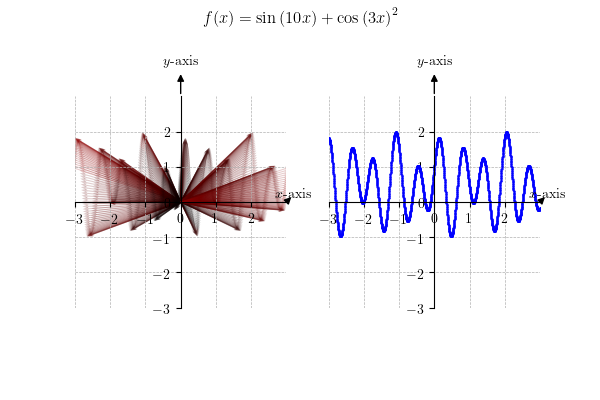
\includegraphics[width=0.8\textwidth]{assets/example1.png}
        \label{fig:example1}
        \caption{On the left, $f$ is represented with 1000 sample vectors. On the right $f$ is shown fully.}
    \end{figure}

    If we were to dot $f$ with another function, say $g(x) = e^x$, it would be nothing more than a point-wise multiplication of our $f$ vector, and then a summation over the interval. The exact value is given by:
    \begin{equation}
        \dfrac{3098\sinh(\pi)}{3737} \approx 9.57398836735
    \end{equation}

    We can instead use the vector forms of $f$ and $g$ to approximate the above. Figure \eqref{fig:example2} displays a visual representation then of $\langle f, g \rangle$:

    This should make sense to any student that has completed a course in elementary calculus: the above sum was nothing more than an approximation of an integral via Riemann sums. The difference here is the data is entirely discretized: no where is a continuous function being used for the above calculations. Instead, we are operating on a discrete approximation of a continuous function, which, in the limit as our sample rate $\to \infty$, becomes therein the continuous function.

    \begin{figure}[h]
        \centering
        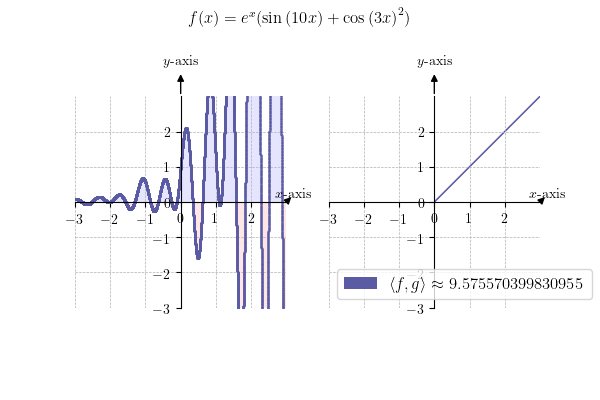
\includegraphics[width=0.8\textwidth]{assets/example2.png}
        \label{fig:example2}

        \caption{On the left, $f \cdot g$ is represented with $40,000$ sample vectors. On the right, the sum of this vector product, multiplied by a factor of $\Delta x = \dfrac{b - a}{N}$ is shown. Notice the error using this approximation is $-1.5\cdot 10^{-3}$.}
    \end{figure}

    \newpage
    Now that we have seen what visual representation of an continuous function's discretized inner product, let's use the same technique to visualize the Fourier transform.
    \label{ex:ex1}
\end{example}

\begin{example}[Fourier Transform Projection]
    Remembering that the Fourier transform was nothing more than simple vector projection, we can illustrate just what that looks like graphically. We'll use the same $f$ as in \eqref{ex:ex1}. First, we'll project a pure complex exponential, $e^{2\pi ix}$ onto $f$, which can be seen in the following figure:

    \begin{figure}[h]
        \centering
        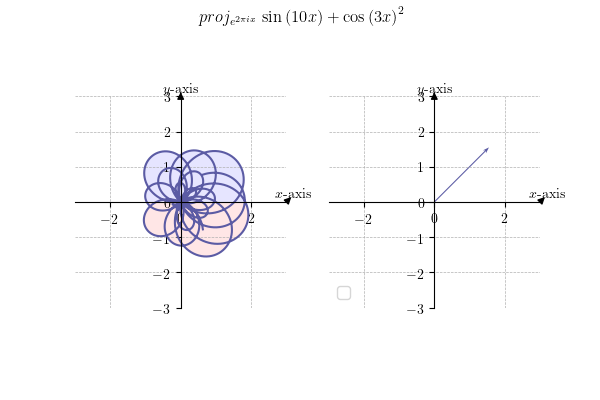
\includegraphics[width=0.8\textwidth]{assets/example3.png}
        \label{fig:example3}
        \caption{}
    \end{figure}
\end{example}


\chapter{The Discrete Fourier Transform}
\label{ch:dft}

Throughout the preceding chapters, we derived the Fourier series and transform for continuous functions in $\mathbf{L}^2$. In practice, however, one works with discrete, finite data. The natural question is: what is the discrete analogue of the Fourier transform? The answer is the Discrete Fourier Transform (DFT), which is not merely an approximation of the continuous transform, but a rich algebraic object in its own right.

\section{DFT as Matrix Multiplication}
\label{sec:dft_matrix}

Given a signal $\vec{x} = (x_0, x_1, \ldots, x_{N-1}) \in \mathbb{C}^N$, the Discrete Fourier Transform produces a vector $\vec{X} = (X_0, X_1, \ldots, X_{N-1})$ defined by:

\begin{definition}[Discrete Fourier Transform]
    \begin{equation}
        X_k = \sum_{n=0}^{N-1} x_n \cdot e^{-2\pi i kn/N}, \quad k = 0, 1, \ldots, N-1
        \label{eq:dft}
    \end{equation}
\end{definition}

Define the $N$th root of unity $\omega_N = e^{-2\pi i/N}$. Then equation \eqref{eq:dft} becomes $X_k = \sum_{n=0}^{N-1} x_n \omega_N^{kn}$, which is precisely a matrix-vector product:

\begin{equation}
    \vec{X} = F_N \vec{x}
\end{equation}

where $F_N$ is the $N \times N$ DFT matrix with entries $(F_N)_{k,n} = \omega_N^{kn}$:

\begin{equation}
    F_N = \begin{pmatrix}
        1      & 1              & 1                  & \cdots & 1                      \\
        1      & \omega_N       & \omega_N^2         & \cdots & \omega_N^{N-1}         \\
        1      & \omega_N^2     & \omega_N^4         & \cdots & \omega_N^{2(N-1)}      \\
        \vdots & \vdots         & \vdots             & \ddots & \vdots                 \\
        1      & \omega_N^{N-1} & \omega_N^{2(N-1)}  & \cdots & \omega_N^{(N-1)^2}
    \end{pmatrix}
\end{equation}

The DFT matrix $F_N$ is symmetric and, up to scaling, unitary: $F_N^{-1} = \frac{1}{N}\overline{F_N}$. This gives us the inverse DFT:

\begin{equation}
    x_n = \dfrac{1}{N}\sum_{k=0}^{N-1} X_k \cdot e^{2\pi i kn/N}
\end{equation}

The connection to the continuous Fourier transform is immediate: as the sampling rate increases ($N \to \infty$ with fixed duration), the DFT converges to samples of the continuous Fourier transform.

\section{The Fast Fourier Transform}
\label{sec:fft}

A direct computation of the DFT requires $O(N^2)$ operations. The Fast Fourier Transform (FFT), discovered by Cooley and Tukey in 1965 \cite{cooley_tukey}, reduces this to $O(N \log N)$ by exploiting the algebraic structure of $\omega_N$.

The key observation is that the DFT of length $N = 2M$ can be decomposed into two DFTs of length $M$:
\begin{align}
    X_k & = \sum_{n=0}^{N-1} x_n \omega_N^{kn}                                                                               \\
        & = \sum_{m=0}^{M-1} x_{2m} \omega_N^{k(2m)} + \sum_{m=0}^{M-1} x_{2m+1} \omega_N^{k(2m+1)}                          \\
        & = \sum_{m=0}^{M-1} x_{2m} \omega_M^{km} + \omega_N^k \sum_{m=0}^{M-1} x_{2m+1} \omega_M^{km}                       \\
        & = E_k + \omega_N^k \cdot O_k
\end{align}

where $E_k$ and $O_k$ are the DFTs of the even-indexed and odd-indexed subsequences, respectively, and $\omega_N^k$ is called the \textit{twiddle factor}. Since $E_k$ and $O_k$ are periodic with period $M$, the ``butterfly'' operation:
\begin{align}
    X_k     & = E_k + \omega_N^k O_k \\
    X_{k+M} & = E_k - \omega_N^k O_k
\end{align}
computes two outputs from each pair. Applying this recursively yields $\log_2 N$ stages of $N/2$ butterflies each, for a total of $O(N \log N)$ operations.

\section{Mixed-Radix and Bluestein's Algorithm}
\label{sec:mixed_radix}

The Cooley-Tukey FFT as presented above requires $N$ to be a power of 2. For arbitrary $N$, two important generalizations exist:

\textbf{Mixed-radix FFT.} If $N = p_1 p_2 \cdots p_k$, the DFT can be decomposed into DFTs of sizes $p_1, p_2, \ldots, p_k$. The most common case is $N = 2^a 3^b 5^c$, supported by FFTW and similar libraries \cite{temperton_mixed}. The complexity remains $O(N \log N)$ provided the prime factors are small.

\textbf{Bluestein's algorithm.} For arbitrary $N$ (including prime $N$), Bluestein's chirp-z transform \cite{bluestein_chirp} converts the DFT into a circular convolution by using the identity:
\begin{equation}
    kn = -\dfrac{(k-n)^2}{2} + \dfrac{k^2}{2} + \dfrac{n^2}{2}
\end{equation}

Substituting into the DFT:
\begin{equation}
    X_k = \omega_N^{k^2/2} \sum_{n=0}^{N-1} \left(x_n \omega_N^{n^2/2}\right) \omega_N^{-(k-n)^2/2}
\end{equation}

This is a convolution of the ``chirped'' signal $x_n \omega_N^{n^2/2}$ with the chirp kernel $\omega_N^{-k^2/2}$, which can be computed via zero-padded FFT of length $\geq 2N-1$ (choosing the next power of 2). The total cost is $O(N \log N)$ regardless of $N$'s factorization.


\chapter{Applications}
\label{ch:applications}

\section{The Convolution Theorem}
\label{sec:convolution}

One of the most powerful results in Fourier analysis is the convolution theorem, which states that convolution in the time domain corresponds to pointwise multiplication in the frequency domain:

\begin{theorem}[Convolution Theorem]
    Let $f, g \in \mathbf{L}^1(\mathbb{R})$. Then:
    \begin{equation}
        \widehat{f * g}(k) = \hat{f}(k) \cdot \hat{g}(k)
    \end{equation}
    where $(f * g)(x) = \int_{-\infty}^{\infty} f(y)g(x - y)\deriv{y}$ is the convolution of $f$ and $g$.
    \label{thm:convolution}
\end{theorem}

\begin{proof}
    \begin{align}
        \widehat{f * g}(k) & = \int_{-\infty}^{\infty} \left[\int_{-\infty}^{\infty} f(y)g(x-y)\deriv{y}\right] e^{-ikx}\deriv{x}     \\
                           & = \int_{-\infty}^{\infty} f(y) \left[\int_{-\infty}^{\infty} g(x-y) e^{-ikx}\deriv{x}\right] \deriv{y}     \\
                           & = \int_{-\infty}^{\infty} f(y) e^{-iky} \hat{g}(k) \deriv{y}                                               \\
                           & = \hat{f}(k) \cdot \hat{g}(k)
    \end{align}
    where the second line follows from Fubini's theorem (interchanging the order of integration), and the third line uses the substitution $u = x - y$.
\end{proof}

The discrete analogue holds for the DFT: circular convolution in the time domain corresponds to pointwise multiplication of DFTs. This is the basis for FFT-based filtering, correlation, and polynomial multiplication.

\section{Image Reconstruction via Epicycles}
\label{sec:epicycles_app}

A striking visual application of Fourier series is the reconstruction of arbitrary closed curves using epicycles---chains of rotating vectors in the complex plane. Given a closed curve $\gamma(t)$, $t \in [0, 1)$, parametrized as a complex-valued function, its Fourier series:
\begin{equation}
    \gamma(t) = \sum_{n=-N}^{N} c_n e^{2\pi int}
\end{equation}
represents $\gamma$ as a sum of $2N + 1$ rotating vectors. Each term $c_n e^{2\pi int}$ traces a circle of radius $|c_n|$ at frequency $n$ rotations per period. Chaining these vectors tip-to-tail, the tip of the last vector traces the reconstructed curve.

The pipeline for reconstructing an arbitrary image as epicycles is:
\begin{enumerate}
    \item \textbf{Edge detection}: extract edges using the Canny algorithm.
    \item \textbf{Contour ordering}: order the edge points into a continuous path via nearest-neighbor traversal.
    \item \textbf{Fourier decomposition}: compute the Fourier coefficients of the complex path.
    \item \textbf{Epicycle rendering}: animate the rotating vectors, tracing the reconstruction.
\end{enumerate}

As $N$ increases, the reconstruction converges to the original contour (by the completeness results of Chapter II). In practice, $N \approx 100\text{--}500$ harmonics suffices for visually faithful reproductions of most images.

\section{Spectral Analysis}
\label{sec:spectral}

The Fourier transform reveals the frequency content of a signal: each coefficient $c_n$ (or $\hat{f}(k)$) encodes the amplitude and phase of the corresponding frequency component. This decomposition is the foundation of spectral analysis.

The \textit{power spectrum} of a signal $f$ is defined as $|c_n|^2$ (discrete) or $|\hat{f}(k)|^2$ (continuous). By Parseval's identity (Theorem \ref{thm:parseval}), the total power is conserved:
\begin{equation}
    \sum_{n=-\infty}^{\infty} |c_n|^2 = \dfrac{1}{2\pi}\int_{-\pi}^{\pi} |f(x)|^2 \deriv{x}
\end{equation}

Applications of spectral analysis include:
\begin{itemize}
    \item \textbf{Audio processing}: identifying the fundamental frequency and harmonics of a musical note.
    \item \textbf{Signal filtering}: removing unwanted frequency components by zeroing their coefficients.
    \item \textbf{Data compression}: retaining only the largest coefficients (lossy compression).
    \item \textbf{Tidal analysis}: decomposing tidal height data into constituent frequencies to predict future tides.
\end{itemize}

In each case, the Fourier transform provides the passage between the time (or spatial) domain and the frequency domain, enabling analysis and manipulation that would be difficult or impossible in the original domain.


\bibliographystyle{plain}
\bibliography{fourier_paper}



\end{document}